\section{Monte Carlo Simulations}


\subsection{Data Generating Process}

In this section, I introduce the \ac{dgp} for the Monte Carlo simulations.
The \ac{dgp} is based on the simulation study by \citet{kang2007demystifying} and \citet{santannaDoublyRobustDifferenceindifferences2020}.
The advantage of this setup is to ensure comparability with previous studies and allowing to validate novel approaches as the use of deep learning for \ac{did} estimation.
For all simulations, the \ac{dgp} has a total sample size of $n=1000$.
There are two time periods $t=0,1$ and two groups $i=0,1$, such that it allows to apply the classical $2\times2$-\ac{did} estimator.
Since individuals are tracked over time, the data is panel data.
\citet{kang2007demystifying} created the \ac{dgp} to include covariate specific trends and homogenous treatment effects.
The true \ac{att} is $\tau = 0$.
In the first simulation shown in Table \ref{tab:table1} I adhere to this specification. In the second simulation in Table \ref{tab:table2} I extend the \ac{dgp} to allow for heterogeneous treatment effects.

To introduce the outcome generation of the \ac{dgp}, consider the arbitrary input vector $M = (M_1, M_2, M_3, M_4)'$ and let the true \ac{or} and propensity score-based \ac{ipw} model be defined as follows:
\begin{align}
    f_{\text{or}}(M) &= 210 + 27.4 \cdot M_1 + 13.7 \cdot (M_2 + M_3 + M_4), \\
    f_{\text{ps}}(M) &= 0.75 \cdot (-M_1 + 0.5 \cdot M_2 - 0.25 \cdot M_3 - 0.1 \cdot M_4).
\end{align}
Note that in this data a selection bias constructed \citep{kang2007demystifying} such that naive estimators are likely to be biased.
As $M$ is arbitrary, \citet{kang2007demystifying} introduce two variations of covariates $Z$ and $X$ that are used in the simulations.
$Z$ is a set of observable variables, while $X$ is a set of unobservable variables.
In this simulation study, $f_{\text{or}}(M)$ and $f_{\text{ps}}(M)$ are constructed only by $Z$, only by $X$, or a combination of both.
Thus there are four different \ac{dgp} setups labeled as DGP1, DGP2, DGP3, and DGP4.
These four setups differ because $Z$ is a non-linear transformation of $X$.

Consider $\mathbf{X} = (X_1, X_2, X_3, X_4)'$ distributed as $N(0, I_4)$, where $I_4$ is the $4 \times 4$ identity matrix.
For $j = 1, 2, 3, 4$, \citet{kang2007demystifying} define the following variations of $Z_j = \frac{\tilde{Z}_j - \mathbb{E}[\tilde{Z}_j]}{\sqrt{\text{Var}(\tilde{Z}_j)}}$ where:
\begin{align} \nonumber
\tilde{Z}_1 &= \exp(0.5X_1), \\ \nonumber
\tilde{Z}_2 &= 10 + \frac{X_2}{1 + \exp(X_1)}, \\
\tilde{Z}_3 &= (0.6 + \frac{X_1 X_3}{25})^3, \quad \text{and} \\ \nonumber
\tilde{Z}_4 &= (20 + X_2 + X_4)^2.  \nonumber
\label{eq:13}
\end{align}
Each variation of $Z$ differs by their functional form as they are quadratic, exponential, and cubic.
They also include variations of interactions of $X$.
This complexity in the functional form of $Z$ is added to invoke potential biases when estimating the \ac{att}.
For example, when the true \ac{dgp} is based on $X$ but the model estimates based on $Z$, then the estimates are likely to be biased.
As we can construct either the \ac{or} or \ac{ipw} model based on $Z$, $X$, or a combination of both, we have four different setups.
The setup for each \ac{dgp} is presented below, indicating which model is correctly specified and which is not.
\begin{multicols}{2}
\textbf{DGP1} \\
(IPW and OR models correct)
\begin{align*}
    Y_0(0) &= f_{\text{or}}(Z) + \nu(Z, D) + \epsilon_0, \\
    Y_1(d) &= 2 \cdot f_{\text{or}}(Z) + \nu(Z, D) + \epsilon_1(d) \\
    p(Z) &= \frac{\exp \left( f_{\text{ps}}(Z) \right)}{1 + \exp \left( f_{\text{ps}}(Z) \right)}, \\
    D &= 1\{ p(Z) \geq U \};
\end{align*}
\textbf{DGP2} \\
(IPW model incorrect, OR correct)
\begin{align*}
    Y_0(0) &= f_{\text{or}}(Z) + \nu(Z, D) + \epsilon_0, \\
    Y_1(d) &= 2 \cdot f_{\text{or}}(Z) + \nu(Z, D) + \epsilon_1(d) \\
    p(X) &= \frac{\exp \left( f_{\text{ps}}(X) \right)}{1 + \exp \left( f_{\text{ps}}(X) \right)}, \\
    D &= 1\{ p(X) \geq U \};
\end{align*}

\columnbreak

\textbf{DGP3}\\
(IPW model correct, OR incorrect)
\begin{align*}
    Y_0(0) &= f_{\text{or}}(X) + \nu(X, D) + \epsilon_0, \\
    Y_1(d) &= 2 \cdot f_{\text{or}}(X) + \nu(X, D) + \epsilon_1(d) \\
    p(Z) &= \frac{\exp \left( f_{\text{ps}}(Z) \right)}{1 + \exp \left( f_{\text{ps}}(Z) \right)}, \\
    D &= 1\{ p(X) \geq U \};
\end{align*}

\textbf{DGP4 } \\
(IPW and OR models incorrect)
\begin{align*}
    Y_0(0) &= f_{\text{or}}(X) + \nu(X, D) + \epsilon_0, \\
    Y_1(d) &= 2 \cdot f_{\text{or}}(X) + \nu(X, D) + \epsilon_1(d) \\
    p(X) &= \frac{\exp \left( f_{\text{ps}}(X) \right)}{1 + \exp \left( f_{\text{ps}}(X) \right)}, \\
    D &= 1\{ p(X) \geq U \};
\end{align*}

\end{multicols}

\subsection{Results Homogenous Treatment Effects}

\begin{table}[htbp]
\centering
\resizebox{\linewidth}{!}{
\begin{threeparttable}
\caption{Monte Carlo Simulation with Homogenous Treatment Effects}
\label{tab:table1}
\begin{tabular}{lllllll}
\toprule
\hline
\addlinespace
Estimator         & Reference                         & Av. Bias   & Med. Bias   & RMSE & Variance & Cover \\ \midrule
\addlinespace
\large \textbf{DGP1}            &                                   &            &             &      &           \\
\addlinespace
$\hat{\tau}^{fe}$ & Regression, Eq. \eqref{eq:twfe}               & -20.963       & -20.816        & 21.277 & 13.247& 0.000      \\
$\hat{\tau}^{corr}$ & Regression, Eq. (2)             & -0.002       & -0.001        & 0.196 & 0.038  &  0.840   \\
$\hat{\tau}^{ipw}$ & Abadie (2005)                    & -0.376       & -0.469        & 9.396 & 45.704 &  0.840      \\
$\hat{\tau}^{ipw,dl}$ & Abadie (2005) + DL            & -3.819       & -3.697        & 3.841 & 36.065 &  1.000    \\
$\hat{\tau}^{dr}$ & Sant'Anna and Zhao (2020)         & 0.003      & 0.008       & 0.218 & 0.022  &  0.834   \\
$\hat{\tau}^{dr,dl}$ & Sant'Anna and Zhao (2020) + DL & -0.121       & -0.120        & 0.121 & 0.020  & 1.000    \\\midrule


\addlinespace
\large \textbf{DGP2}            &                                   &            &             &      &           \\
\addlinespace
$\hat{\tau}^{fe}$ & Regression, Eq. \eqref{eq:twfe}               & -19.261      & -19.040      & 19.606 & 13.403 & 0.000      \\
$\hat{\tau}^{corr}$ & Regression, Eq. (2)             & -0.004       & -0.001        & 0.195 & 0.038  & 0.832     \\
$\hat{\tau}^{ipw}$ & Abadie (2005)                    & -0.498       & -0.472        & 9.660 & 47.106  & 0.839    \\
$\hat{\tau}^{ipw,dl}$ & Abadie (2005) + DL            & -21.983       & -22.114        & 22.335 & 43.872 & 0.000    \\
$\hat{\tau}^{dr}$ & Sant'Anna and Zhao (2020)         & 0.005       & 0.002        & 0.207 & 0.021  & 0.802    \\
$\hat{\tau}^{dr,dl}$ & Sant'Anna and Zhao (2020) + DL  & -0.148       & -0.150        & 0.148 & 0.020  &  1.000    \\  \midrule


\addlinespace
\large \textbf{DGP3}            &                                   &            &             &      &           \\
\addlinespace
$\hat{\tau}^{fe}$ & Regression, Eq. \eqref{eq:twfe}               & 13.122       & 12.899       & 14.028 & 24.575 & 0.109    \\
$\hat{\tau}^{corr}$ & Regression, Eq. (2)             & 0.142       & -0.114       & 4.869 & 23.685 &0.782   \\
$\hat{\tau}^{ipw}$ & Abadie (2005)                    & 0.109     & 0.219      & 9.630 & 43.498  & 0.817   \\
$\hat{\tau}^{ipw,dl}$ & Abadie (2005) + DL            & -0.810       & -0.794        & 0.824 & 40.227  &   1.000  \\
$\hat{\tau}^{dr}$ & Sant'Anna and Zhao (2020)         & -0.104       & 0.052        & 4.599 & 11.165  &0.840    \\
$\hat{\tau}^{dr,dl}$ & Sant'Anna and Zhao (2020) + DL & 0.228       & 0.219        & 0.293 & 11.240   &1.000   \\  \midrule


\addlinespace
\large \textbf{DGP4}            &                                   &            &             &      &           \\
\addlinespace
$\hat{\tau}^{fe}$ & Regression, Eq. \eqref{eq:twfe}              & -16.434       & -16.283        & 17.226 & 26.633  & 0.033   \\
$\hat{\tau}^{corr}$ & Regression, Eq. (2)             & -3.063       & -3.165       & 6.162 & 28.588  &0.654   \\
$\hat{\tau}^{ipw}$ & Abadie (2005)                    & -3.881       & -4.063        & 10.576 & 47.230    & 0.798  \\
$\hat{\tau}^{ipw,dl}$ & Abadie (2005) + DL            & -4.992       & -4.962        & 5.005 & 43.947 & 1.000     \\
$\hat{\tau}^{dr}$ & Sant'Anna and Zhao (2020)         &-3.177      &-3.162       & 5.899 & 12.259  &0.752    \\
$\hat{\tau}^{dr,dl}$ & Sant'Anna and Zhao (2020) + DL & 1.630       & 1.593        & 1.652 & 15.876  &1.000    \\


\bottomrule
\end{tabular}
\vspace{1em}
\begin{tablenotes}
\item Notes: Simulations based on panel data with sample size $n = 1000$ and 1000 Monte Carlo repetitions. The average bias "Av. Bias", median bias "Med. Bias", root mean squared error "RMSE", and average variance "Variance" of the estimators are reported. The "Cover" describes the coverage probability of how often the estimated treatment coefficient falls within the confidence intervall of the true treatment effect. The methods that predict propensity scores with deep learning are marked by "DL". The true treatment effect is $\tau = 0$ in all cases and homogenous.
\end{tablenotes}
\end{threeparttable}}
\end{table}


In this section I present the results of the Monte Carlo simulations for the homogenous treatment effects case.
Table \ref{tab:table1} and Table \ref{tab:table2} report the average bias, median bias, root mean squared error, and variance of the estimators.
$\hat{\tau}^{corr}$ are the results of the correctly specified \ac{twfe} from Equation \ref{eq:twfecorr}, which can be interpreted as a baseline for the other estimators.
$\hat{\tau}^{fe}$ is the naive \ac{twfe} estimator from Equation \ref{eq:twfe}, as argued, the estimator is highly biased because the naive selection of controls does not reflect the underlying function of the data.
Note that the coverage probability is across \ac{dgp}s almost zero.
$\hat{\tau}^{ipw}$ and $\hat{\tau}^{dr}$ are the results of the \ac{ipw} and \ac{drdid} estimators, respectively.
In both cases are the propensity scores estimated with a logistic regression.
The results of $\hat{\tau}^{fe}$, $\hat{\tau}^{ipw}$, and $\hat{\tau}^{dr}$ are directly comparable to the results of \citet{santannaDoublyRobustDifferenceindifferences2020} panel data case.
$\hat{\tau}^{ipw,dl}$ and $\hat{\tau}^{dr,dl}$ are the results of the \ac{ipw} and \ac{drdid} estimators, respectively, where the propensity scores are estimated with a neural network.
Note that the \ac{or} part of $\hat{\tau}^{dr,dl}$ is estimated as a linear model.

One can see that in DGP1 all estimators have relatively small biases, except for the naive \ac{twfe} estimator.
Also the coverage is quite high, and reaches in the case of the deep learning applications even 1.
This is most likely due to inflated confidence interval length \citep{farrellDeepNeuralNetworks2021}.
This is consistent as DGP1 marks the case where the \ac{ipw} and \ac{or} models are correctly specified.
In DGP2 the propensity score approach is misspecified such that $\hat{\tau}^{ipw}$ and $\hat{\tau}^{ipw,dl}$ are biased but the bias for the  $\hat{\tau}^{ipw,dl}$ is substantial.
Possible reasons could be overfitting or the prediction of extreme propensity scores.
Generally does the approach \ac{ipw} model approach produce high variance which is consistent with \citet{santannaDoublyRobustDifferenceindifferences2020} and seem to be also the case for other data structures like repeated cross-section \citep{santannaDoublyRobustDifferenceindifferences2020,manfeDifferenceInDifferenceDesignRepeated}.
On the other hand in DGP3 one can clearly see that all estimators are relatively unbiased, except for the naive \ac{twfe} estimator as before.
These results are consistent as DGP3 marks the case where the \ac{ipw} model is correctly specified.
In DGP1-3 are both \ac{drdid} estimators $\hat{\tau}^{dr}$ and $\hat{\tau}^{dr,dl}$ relatively unbiased and produce low variance.
Notably the classic $\hat{\tau}^{dr}$ of \citet{santannaDoublyRobustDifferenceindifferences2020} does perform slightly better.

DGP4 is the most challenging but probably most realistic case as both the \ac{ipw} and \ac{or} models are misspecified.
One can see clearly that all estimators are now more biased and have higher variance.
Surprisingly is that the $\hat{\tau}^{dr,dl}$ reports the smallest bias and relatively small variance compared to the other estimators.
This result is consistent with the findings of \citet{belloni2017program,chernozhukovDoubleDebiasedMachine2018,farrellDeepNeuralNetworks2021} that deep learning is useful to recover the true treatment effect if there is nuisance in the data.



Overall, the results seem to be consistent with the findings of the literature of deep learning and \ac{did} estimation.
It should be noted that the biases of the deep learning estimators are relatively similar distributed within each \ac{dgp}.
This indicates that the deep learning models results across the monte carlo runs is consistent and not heavily driven by outliers.
The results are also mirroring a structural aspect of deep learning that especially when using regularization methods they are prone to produce symmetrically distributed errors around zero \citep{koh2017understanding}.

To evaluate if the deep learning model is robust, I report the minimum loss of the training and validation set in Table \ref{tab:table3}.
Note that I implement one model and applied it on all \ac{dgp} setups, such that the results are comparable.
Across all \ac{dgp} setups the deep learning model reports similar losses, indicating that the model itself leads to the results shown and not the variability in the data.
Importantly, across all setups is the validation loss smaller than the training loss, indicating that the model is not overfitting \citep[see][]{Goodfellow-et-al-2016,farrellDeepNeuralNetworks2021}.


%discuss consistency of results with other papers sant anna
%bad performance of abadie dl. Discuss!
%dl performs worse except in the case of dgp4. Discuss!
%why are the biases of dl so similiar distributed? Discuss!


% Please add the following required packages to your document preamble:
% \usepackage{booktabs}
% Please add the following required packages to your document preamble:
% \usepackage{booktabs}
\begin{table}[ht]
\centering
\begin{threeparttable}
\caption{Performance of the Neural Network across DGPs}
\label{tab:table3}
\begin{tabular}{ccccc} %\begin{tabular}{@{}lllll@{}}
\toprule
\hline
\addlinespace
Minimum Loss  & DGP1 & DGP2 & DGP3 & DGP4 \\ \midrule
Training   & 0.634 & 0.631 & 0.634 & 0.632 \\
Validation  & 0.617 & 0.626 & 0.617 & 0.625 \\ \bottomrule
\end{tabular}
\begin{tablenotes}
    \item Notes: The neural networks width is set to 32. The depth is set to 3 and the learning rate is set to 0.01. The number of epochs to 50. This specifications are set across all DGPs for the same neural network.
\end{tablenotes}
\end{threeparttable}
\end{table}



\subsection{Results Heterogeneous Treatment Effects}
In previous section I outlined the advantage of neural networks, or machine learning in general, when dealing with heterogenous treatment effects.
The problem of heterogenous treatment effect arises when the treatment effect $\theta(X)$ varies \citep{hansen2022econometrics}.
To validate how the aforementioned estimators perform under heterogenous treatment effects I introduced heterogeneity to the DGP4.
DGP4 is the most general and possibly the most realistic case of the observed \ac{dgp}s.
The main difference to the DGP4 with homogenous treatment effects is the introduction of $\theta(X)$, which directly influences the outcome $Y_1(d)$ depending on the value of $X$.
\\
\textbf{DGP4 with Heterogeneous Treatment Effects}
\begin{align*}
    Y_0(0) &= f_{\text{or}}(X) + \nu(X) + \epsilon_0, \\
    Y_1(d) &= 2 \cdot f_{\text{or}}(X) + \nu(X) + \theta(X) \cdot d + \epsilon_1(d), \\
    p(X) &= \frac{\exp \left( f_{\text{ps}}(X) \right)}{1 + \exp \left( f_{\text{ps}}(X) \right)}, \\
    D &= 1\{ p(X) \geq U \},
\end{align*}
where: $\theta(X) = 10 \cdot (Z_1 + Z_2 - Z_3 + Z_4)$.\\
\begin{table}[]
\centering
\begin{threeparttable}
\caption{Monte Carlo Simulation with Heterogenous Treatment Effects in DGP4}
\label{tab:table2}
\begin{tabular}{lllllll}
\toprule
\hline
\addlinespace
Estimator         & Reference                         & Av. Bias   & Med. Bias   & RMSE & Variance & Cover \\ \midrule
\addlinespace
$\hat{\tau}^{fe}$ & Regression, Eq. \eqref{eq:twfe}               & -20.418      & -20.245        & 21.242 & 34.360  &0.015   \\
$\hat{\tau}^{corr}$ & Regression, Eq. \eqref{eq:twfecorr}           & -9.429      & -9.355       & 10.602 & 23.483  &0.225  \\
$\hat{\tau}^{ipw}$ & Abadie (2005)                    & -7.866       & -7.899       & 13.231 & 55.196   &0.712  \\
$\hat{\tau}^{ipw,dl}$ & Abadie (2005) + DL            & -8.424       & -8.408        & 8.432 & 51.123   &1.0   \\
$\hat{\tau}^{dr}$ & Sant'Anna and Zhao (2020)         & -7.238      & -7.128        & 10.115 & 24.060   & 0.619   \\
$\hat{\tau}^{dr,dl}$ & Sant'Anna and Zhao (2020) + DL & -1.596       & -1.607        & 1.633 & 16.570   & 1.0  \\

\bottomrule
\end{tabular}
\begin{tablenotes}
    \item Notes: Simulations based on panel data with sample size $n = 1000$ and 1000 Monte Carlo repetitions. The average bias "Av. Bias", median bias "Med. Bias", root mean squared error "RMSE", and average variance "Variance" of the estimators are reported. The methods that predict propensity scores with deep learning are marked by "DL". The true treatment effect is $\tau = 0$ and heterogenous in all cases.
\end{tablenotes}
\end{threeparttable}
\end{table}

The results of the Monte Carlo simulations with heterogenous treatment effects are presented in Table \ref{tab:table2}.
The estimators $\hat{\tau}^{fe}$,$\hat{\tau}^{corr}$,$\hat{\tau}^{ipw}$, and $\hat{\tau}^{dr}$ are now more biased and have higher variance compared to the homogenous treatment effects case.
These results are consistent with the literature as these methods do not account for heterogeneity \citep{hansen2022econometrics}.
\citet{manfeDifferenceInDifferenceDesignRepeated} reports similar more biased results for the \ac{ipw} and \ac{drdid} estimator in the case of repeated cross-section data.
The $\hat{\tau}^{ipw,dl}$ also reports higher bias and variance compared to the homogenous treatment effects case.
But overall is the bias and variance now smaller than the comparable $\hat{\tau}^{ipw}$.
The same is true for the $\hat{\tau}^{dr,dl}$, which reports the smallest bias and variance across all estimators.
These results are interestingly as it indicates that neural networks are more robust towards covariate specific trends and heterogenous treatment effects than comparable estimators in this thesis.
This is consistent with the findings of \citet{farrellDeepNeuralNetworks2021} and \citet{chernozhukovDoubleDebiasedMachine2018}.

\subsection{Comparison of Deep Learning Architectures}

The choice of the correct neural network is generally arbitrary as discussed in Section 3.
This is due to the chosen activation function is chosen, neural network class or hyperparameters.
Table \ref{tab:nn} shows the influence of different hyperparameters on the \ac{dgp} used in Section 4.3.
Note that the activation function is \ac{relu} and the neural network is a feedforward neural network across all architectures.

It is clear to see in table \ref{tab:nn} that there is no strictly better alternative architecture comparing these neural network class.
Every change in the  hyperparameter selection comes to the cost of either higher bias or higher variance, which is a common trade-off in machine learning.
For example has the classic architecture higher bias than the first variation that has more hidden layers and units.
This comes to the cost of higher variance.
Interestingly is there no clear sign that deeper neural networks (with more units and layers) actually imposes better results than shallower networks.
Generally come deeper neural networks with higher computational costs, which can be extensive especially in case of complex and large data.

Additionally one can see that the first variation of the architecture has a bigger validation loss than training loss.
The neural networks 4 and 5 report very small differences between the losses.
As argued indicates a higher validation loss to training that the model overfits.
For practioners it might be useful to use the results of the loss to evaluate which neural networks to select.
\begin{table}[ht]
\centering
\resizebox{\linewidth}{!}{
\begin{threeparttable}
\caption{Simulation Results across Neural Network Architectures}
\label{tab:nn}
\begin{tabular}{lrrrrrr}
    \toprule
\hline
\addlinespace
Metric \textbackslash Architecture & Classic &  1 &  2 &  3 &  4 &  5 \\
\addlinespace
\hline
\addlinespace
Avg Bias & -1.5726 & -0.0419 & -2.7408 & -6.0963 & -6.1169 & -4.4494 \\
Med Bias & -1.6320 & -0.4206 & -2.6777 & -6.1525 & -6.2021 & -4.5586 \\
RMSE & 1.6130 & 1.4939 & 2.7739 & 6.0976 & 6.2239 & 4.4667 \\
Variance & 16.5906 & 20.9828 & 15.8893 & 10.9668 & 11.0447 & 11.7120 \\
Training Loss & 0.6316 & 0.6083 & 0.6270 & 0.6585 & 0.7217 & 0.6573 \\
Validation Loss & 0.6252 & 0.6209 & 0.6193 & 0.6554 & 0.7203 & 0.6513 \\
Avg Coverage Prob & 1.0000 & 1.0000 & 1.0000 & 1.0000 & 0.5000 & 1.0000 \\
\addlinespace
\hline
\addlinespace
Depth & 3 & 5 & 2 & 3 & 3 & 6 \\
Units & 32 & 64 & 16 & 128 & 16 & 128 \\
Learning Rate & 0.01 & 0.001 & 0.01 & 0.001 & 0.0001 & 0.001 \\
L2 Regularization & 0.01 & 0.001 & 0.01 & 0.1 & 0.01 & 0.01 \\
\hline
\end{tabular}
\begin{tablenotes}
    \item aojwdb
\end{tablenotes}
\end{threeparttable}}
\end{table}


Observing the coverage probability in Table \ref{tab:nn} one can see again the extreme coverage of 1 in all but one case.
The exemption variation 4 has the lowest learning rate and reports coverage probability of 0.84.
The learning rate is comparable to \citet{farrellDeepNeuralNetworks2021} that also report very high coverage probabilites but not as extreme as here.
%regularization preach cautios
%say something theoretically about learning rates here
To better understand why in the most cases here the coverage probabilities reported here are extreme one can observe figure \ref{fig:atte_bounds}.
Over all 1000 runs of the \ac{mcs} the estimated conditional \ac{att} never reaches the smallest upper or lower bound.
Interestingly the true zero effect is never recovered.
The very dense and narrow distribution is comparable to the results of \citet{farrellDeepNeuralNetworks2021}.

These results show that there is still no clear understanding how to select optimal deep learning models for inference.
The comparison of the neural network architectures even implies a modest sensitivity towards selected hyperparameters.
There are options like grid search with frameworks like TensorFlow\textsuperscript{\textregistered} that can help in selecting hyperparameters for simulations but for observational data the choice of optimal neural networks remains unclear.
\\
\begin{figure}[h]
\centering
\caption{Conditional Average Treatment on the Treated Effekt with Bounds}
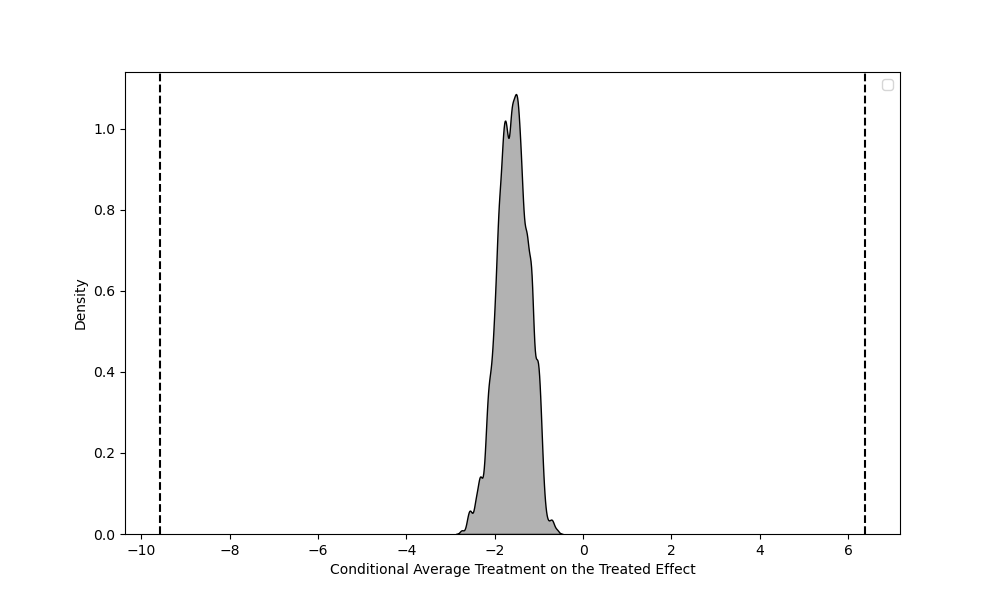
\includegraphics[width=\textwidth]{atte_bounds}
\label{fig:atte_bounds}
\end{figure}
